\section{ASEC Inverse Secant Function}

\subsection{Usage}

Computes the inverse secant of its argument.  The general
syntax for its use is
\begin{verbatim}
  y = asec(x)
\end{verbatim}
where \verb|x| is an \verb|n|-dimensional array of numerical type.
\subsection{Function Internals}

The \verb|acosh| function is computed from the formula
\[
   \sec^{-1}(x) = \cos^{-1}\left(\frac{1}{x}\right)
\]
\subsection{Examples}

Here is a simple plot of the inverse secant function
@>


\centerline{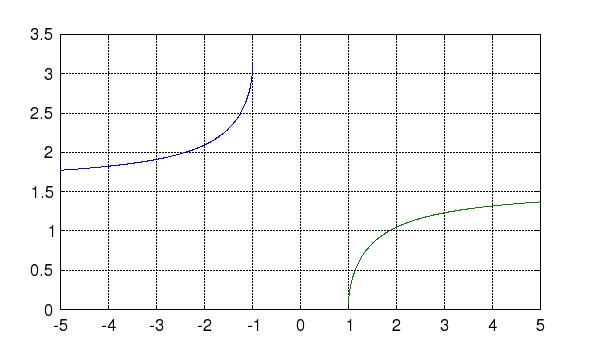
\includegraphics[width=8cm]{asecplot}}

